% ###########################################################################
% #### The NorNet Handbook                                               ####
% #### Copyright (C) 2012-2015 Thomas Dreibholz                          ####
% ###########################################################################

% @@@@@@@@@@@@@@@@@@@@@@@@@@@@@@@@@@@@@@@@@@@@@@@@@@@@@@@@@@@@@@@@@@@@@@@@@@@
\chapter{Basics}
\label{cha:Basics}
% @@@@@@@@@@@@@@@@@@@@@@@@@@@@@@@@@@@@@@@@@@@@@@@@@@@@@@@@@@@@@@@@@@@@@@@@@@@

% ###########################################################################
\section{Introduction}
\label{sec:Introduction}
% ###########################################################################

The Internet has quickly become a critical infrastructure that our modern society heavily relies on. No longer is the Internet only a carrier of less time- and availability-critical services like e-mail and file transfer, but it now also carries services like e.g.\ e-commerce and healthcare, where even a temporary disruption of service could result in huge economical losses, reduced quality of healthcare or even death in the extreme cases. Failures, however, are unavoidable, and our current Internet needs to be improved to ensure the availability of critical services even when the underlying network fails. One way of doing this is to increase resilience through the use of \emph{multi-homing}. A multi-homed node is connected to more than one \emph{Internet Service Provider}~(ISP), in order to improve availability through the use of multiple Internet connections. As long as at least one ISP is operational, the node and its services should remain available.

The size and complexity of the Internet, together with the increased use of the network as a carrier for critical services, is a barrier for doing changes to the current infrastructure of the network. New ideas, like new protocols and algorithms related to multi-homing, need to be thoroughly tested and verified before they can be deployed. Furthermore, the testing and verification needs to be conducted in a realistic environment for the results to be valid. To satisfy this need in the context of multi-homing, we are realising the distributed multi-homed testbed \noun{NorNet}. Particularly, it will be the first testbed platform that provides the possibility to perform realistic and large-scale multi-homing experiments in the Internet.

The goal of this chapter -- based on~\cite{PAMS2013-NorNet,ComNets2013-Core} -- is to introduce the \noun{NorNet} testbed to the reader. Therefore, the chapter will give a general overview of the testbed, and a detailed description of the design and implementation of the fixed-line part of it, \noun{NorNet Core}. By sharing the implementation details of \noun{NorNet Core} and informing about the capabilities of the testbed, we would like to invite researchers in multi-homing to become future users of the \noun{NorNet} testbed.



% ###########################################################################
\section{The Design}
\label{sec:Design}
% ###########################################################################

The \noun{NorNet} testbed is made up of two parts, \noun{NorNet Edge} and \noun{NorNet Core}. \noun{NorNet Edge} is the wireless part of the \noun{NorNet} infrastructure. It consists of more than 500~multi-homed measurement nodes that are geographically distributed in Norway, each node being connected to five wireless broadband ISPs. \noun{NorNet Core}, on the other hand, which is the main subject of this chapter, consists of a set of multi-homed, programmable sites being interconnected by wired Internet connections.

Figure~\ref{cap:NorNet-Sites-Map} shows the location of the ten first \noun{NorNet Core} sites. Each site consists of four servers and a switch, where one of the servers acts as a so-called \emph{tunnelbox}. While the switch connects all the servers, or \emph{nodes}, locally at a site, the tunnelbox is responsible for connecting its own site to other sites in \noun{NorNet Core}, by using the available set of ISPs (see Figure~\ref{cap:NorNet-Network}). Note that a tunnelbox creates connections, or more precisely IPv4 and IPv6 \emph{tunnels}, by using all possible combinations of local ISPs and remote ISPs at all the other sites' tunnelboxes. That is, the topology of the \noun{NorNet Core} is a fully connected mesh. At each site, \noun{Uninett} (the ISP for the Norwegian research institutions) is used as the default ISP for all administrative purposes.

The additional servers at the sites, that is, the ones not being tunnelboxes, host the virtual resources that are made available for researchers to perform experiments in \noun{NorNet Core}. While there are currently three such servers at each site, it is of course possible to extend their number if there is need for increased research resources. The administration of resources and users is realised by using a private \noun{PlanetLab}~\cite{PBF+05} installation, with a central server located at the Simula Research Laboratory~\cite{SimulaBook} site. Resources are then requested and provided to the researchers as \emph{slices}. A key challenge of the original \noun{PlanetLab} testbed is the low availability of nodes. At the time this section was written, only about~36\% of the \noun{PlanetLab} member nodes were actually available\footnote{We have associated all 1,035~registered nodes to a test slice but were able to login to only~367, i.e.\ about~36\%, of them. Test made on June~28, 2012.} for usage. To avoid a similar situation in \noun{NorNet Core}, a close monitoring and administrative scheme is enforced throughout the testbed. 

% %%%%%%%%%%%%%%%%%%%%%%%%%%%%%%%%%%%%%%%%%%%%%%%%%%%%%%%%%
\begin{figure}
\begin{center}
\includegraphics[width=0.80\columnwidth]{Figures/PDF/Norway_noLinks_inkl_Svalbard.pdf}
\end{center}
\caption{The \noun{NorNet Core} Sites Map}
\label{cap:NorNet-Sites-Map}
\end{figure}
% %%%%%%%%%%%%%%%%%%%%%%%%%%%%%%%%%%%%%%%%%%%%%%%%%%%%%%%%%

% %%%%%%%%%%%%%%%%%%%%%%%%%%%%%%%%%%%%%%%%%%%%%%%%%%%%%%%%%
\begin{figure}
\begin{center}
\includegraphics[width=0.80\columnwidth]{%
   Figures/PDF/NorNetCore-Network.pdf}  
\end{center}
\caption{The \noun{NorNet Core} Network Schema}
\label{cap:NorNet-Network}
\end{figure}
% %%%%%%%%%%%%%%%%%%%%%%%%%%%%%%%%%%%%%%%%%%%%%%%%%%%%%%%%%



% ###########################################################################
\section{The Implementation}
\label{sec:Implementation}
% ###########################################################################

In the following, we describe the implementation of the fixed-line \noun{NorNet Core} testbed.


% ===========================================================================
\subsection{The Testbed Management}
\label{sub:The-Testbed-Management}
% ===========================================================================

\noun{NorNet Core} intends to reuse the \noun{PlanetLab}~\cite{PBF+05} software whenever possible. This software is available in a couple of distributions, most notably the original \noun{PlanetLab} software itself as well as \noun{OneLab}\footnote{\noun{OneLab}: \url{http://www.onelab.eu/}.}. All variants have in common that there is a central administration component, denoted as \emph{PlanetLab Central}~(PLC)~\cite{Hua06}. The PLC manages a database with the configurations of sites, nodes, users and slices. Also, it provides a web-based administration interface as well as an XMLRPC-based API -- called PLCAPI~\cite{PLCAPI} -- for software-based access to the configuration database. A particularly useful feature of the PLC software is to allow for custom extensions by adding so-called \emph{tags} to the database. Tags are additional information to be managed, like e.g.\ testbed-specific configuration parameters.

For \noun{NorNet Core}, it has been straightforward to reuse the PLC as a basis. Custom, \noun{NorNet}-specific configuration is simply realised by appropriate tags. In particular, tags are used to store additional information about the tunnelbox configurations (ISPs, addresses, etc.) and provider networks available at each site. The PLCAPI allows the \noun{NorNet} components -- which will be introduced later -- to access their configuration information and apply it as needed.


% ===========================================================================
\subsection{The Sites}
\label{sub:The-Sites}
% ===========================================================================

% %%%%%%%%%%%%%%%%%%%%%%%%%%%%%%%%%%%%%%%%%%%%%%%%%%%%%%%%%
\begin{figure}
\begin{center}
\subfigure[Schematic View]{
\includegraphics[height=6.00cm]{%
   Figures/PDF/NorNetCore-Site-PhysicalSetup.pdf}  
\label{subcap:Setup-Schema}
}
\subfigure[A Real Deployment]{
\includegraphics[height=6.00cm]{%
   Images/PDF/NorNetCore-Tromsoe.pdf}
\label{subcap:Setup-Real}
}
\end{center}
\caption{The Physical Site Setup}
\label{cap:The-Site-Setup}
\end{figure}
% %%%%%%%%%%%%%%%%%%%%%%%%%%%%%%%%%%%%%%%%%%%%%%%%%%%%%%%%%

Each \noun{NorNet Core} site needs appropriate hardware to realise routing (i.e.\ the tunnelbox functionality) as well as to provide resources for researchers. Therefore, we have decided to deploy the setup depicted in Figure~\ref{cap:The-Site-Setup} at each site; Subfigure~\ref{subcap:Setup-Schema} shows a schematic illustration of a site, while subfigure~\ref{subcap:Setup-Real} shows a picture of a real setup\footnote{Setup at Universitetet i Tromsø~(UiT), Troms/Nord-Norge.}.
A site physically consists of one managed switch and four HP~DL320 servers. All servers have an identical configuration (4-core x86\_64-CPU, 8~GiB RAM, ca.\ 500~GiB harddisk, and two 1000BaseT Ethernet interfaces). Since server~1 (figure~\ref{subcap:Setup-Schema}) is intended to work as a tunnelbox, it also contains an additional network interface card with four 1000BaseT Ethernet ports. The first of these ports is connected to \noun{Uninett}; the other ports are used for further providers (not yet connected in the depicted setup). The switch connects the first built-in Ethernet port of the servers~1 to~4. This Ethernet hosts the \noun{NorNet}-internal, provider-specific networks (which are realised by Ethernet VLANs).

The operating system installed on the servers is \noun{Ubuntu Linux}\footnote{\noun{Ubuntu Linux}: \url{http://www.ubuntu.com/}.} 12.04~LTS, a version with five years support, realised as a quite minimal server installation (to be explained in more detail in Subsection~\ref{sub:The-Software}). The purpose of this installation is to allow for basic configuration tasks, remote login by using \emph{Secure Shell}~(SSH)~\cite{RFC4254} as well as to run \noun{VirtualBox}~\cite{VirtualBoxUserManual} to host virtual machines for all further tasks. Particularly, this means that the tunnelbox, a control system (allowing remote debugging and configuration tasks) and all research systems are realised as virtual machines. This allows for a good utilisation of the available hardware resources, and it is furthermore possible to add and remove systems on demand (e.g.\ for testing, for special kernel-based experiments not being possible with the \noun{PlanetLab} software, etc.). Also, it allows to easily backup and restore the virtual systems, without requiring physical access to the hardware itself. This should make it possible to resolve most problems \emph{quickly}, in order to achieve minimal downtime for the testbed users.

To provide access to a site even when server 1 (hosting the tunnelbox and therefore handling routing to other \noun{NorNet Core} sites and the Internet) is not working properly, the control system on the fourth server is also equipped with a global IP~address in the \noun{Uninett} network (not yet connected in Subfigure~\ref{subcap:Setup-Real}).

For fast deployment, the \noun{Ubuntu Linux} setup for the machines has been preseeded on an installation USB-stick. Preseeding~\cite{UbuntuServerGuide} denotes to automatically apply a pre-defined configuration, i.e.\ partitioning the harddisk, selecting software packages and performing post-installation configuration tasks. That is, to install a server, the only manual tasks are to set up the network and to confirm repartitioning. Once server 1 is able to perform routing, the three other servers can run the installation procedure in parallel. Network access during installation is necessary to ensure up-to-date package versions (including security updates).

While all sites host virtual machines with one tunnelbox, a control system and some research systems (to be explained in detail in Subsection~\ref{sub:The-Research-Systems}), the Central Site -- at the Simula Research Laboratory (see the map in Figure~\ref{cap:NorNet-Sites-Map}) -- also hosts the PLC server (see Subsection~\ref{sub:The-Testbed-Management}) as well as the network monitoring infrastructure (to be introduced in Subsection~\ref{sub:The-Monitoring-Setup}). Also, a file server is available to store virtual machine image backups.


% ===========================================================================
\subsection{The Software}
\label{sub:The-Software}
% ===========================================================================


\noun{Ubuntu Linux}, as a variant of \noun{Debian Linux}, is based on the package manager \emph{Advanced Packaging Tool}~(APT)~\cite{DebianDevelopersReference}. The \noun{Debian} tool-chain allows for easy creation, validation and building of software packages, including automatic handling of software dependencies, where the packages can be provided in a software repository for download. For \noun{Ubuntu}, there is a cloud service provided for this task on \noun{Launchpad}\footnote{\noun{Launchpad}: \url{http://www.launchpad.net/}.}: \emph{Personal Package Archives}~(PPA). Using PPA, it is just necessary to create a source package and upload it into this cloud service. It will then automatically build binary installation packages, which are afterwards provided in a package repository. Since this service has shown to be very convenient, it is also applied for \noun{NorNet Core}. All \noun{NorNet Core} systems just need to refer to the PPA for package installation, in order to obtain the up-to-date \noun{NorNet Core} software.
Furthermore, the APT-based packaging with its support for automatic dependency resolution allows to efficiently break down a larger software system, like \noun{NorNet Core}, into multiple packages. The \noun{NorNet Core} packages are depicted in Figure~\ref{cap:The-Software-Packages}. Please refer to this figure while reading about the packages in the following sections.
% ; they will be introduced in the following subsections.

% %%%%%%%%%%%%%%%%%%%%%%%%%%%%%%%%%%%%%%%%%%%%%%%%%%%%%%%%%
\begin{figure*}
\begin{center}
\includegraphics[width=0.80\columnwidth]{%
   Figures/PDF/NorNetCore-Packages.pdf}
\end{center}
\caption{The Software Packages}
\label{cap:The-Software-Packages}
\end{figure*}
% %%%%%%%%%%%%%%%%%%%%%%%%%%%%%%%%%%%%%%%%%%%%%%%%%%%%%%%%%


% ===========================================================================
\subsection{The Physical Servers}
% ===========================================================================

The installation of a physical server (see Subsection~\ref{sub:The-Sites}) is described by the meta-package ``Server''. It is automatically installed by the preseed procedure and particularly ensures the installation of \noun{VirtualBox}~\cite{VirtualBoxUserManual} for the virtualisation, plus system management tools.
These added system management tools include e.g.\ \noun{Traceroute} (routing debugging), \noun{Whois} (IP ownership query tool), \noun{SubNetCalc}\footnote{\noun{SubNetCalc}: \url{http://www.iem.uni-due.de/~dreibh/subnetcalc/}.} (IP network calculator), \noun{NetPerfMeter}~\cite{SoftCOM2011} (advanced network performance metering tool), \noun{rsplib}~\cite{Dre2006} tools (RSerPool debug tools), \noun{OpenSSH} (SSH server for remote login~\cite{RFC4254}), SNMP tools (for accessing network management information~\cite{RFC3411}) and \noun{GPM}\footnote{\noun{GPM}: \url{http://www.nico.schottelius.org/software/gpm/}.} (mouse support for the console). Since these tools are not only useful for physical servers, they have been grouped in the meta-package ``Management''. It will be installed as a dependency of the ``Server'' package.


% ===========================================================================
\subsection{The Virtual Nodes}
\label{sub:The-Nodes}
% ===========================================================================

All standard virtual \noun{NorNet Core} systems run \noun{Ubuntu Linux} and are based on the ``Node'' package. Similar to ``Server'', it depends on ``Management'' to install the system management tools. Also, ``Node''-based systems need to access the PLCAPI (see Subsection~\ref{sub:The-Testbed-Management}). To make it easier to use the \noun{NorNet}-specific extensions (stored as tags), the ``API'' package contains some \noun{Python} classes and scripts for that purpose.

In addition, the ``Node'' package installs some management scripts. Particularly, \noun{cron-apt}\footnote{\noun{cron-apt}: \url{http://inguza.com/software/cron-apt}.} will be set up to automatically apply APT-based package updates, in order to keep the installation up-to-date. Also, a \noun{cron}-job is installed to regularly query the PLC database for configuration changes. Once there is a configuration update, it will be applied. The following configuration tasks are handled in this way:
\begin{itemize}
 \item The hostname of the system is set.
 \item The IP configuration of the \noun{NorNet}-internal networks is applied.
 \item \emph{Domain Name System}~(DNS)~\cite{RFC1035} server addresses are set.
 \item The \emph{Network Time Protocol}~(NTP) service for time synchronisation is configured (to be explained in Subsection~\ref{sub:The-Tunnelboxes}).
 \item The \emph{Simple Network Management Protocol}~(SNMP)~\cite{RFC3411} service is set up. It allows to query status information of the system within the \noun{NorNet}-internal network. Particularly, it will be used for monitoring (to be explained in Subsection~\ref{sub:The-Monitoring-Setup}).
\end{itemize}

Also, the ``Node'' package installation updates the configuration of the \noun{Grub2} boot manager. Particularly, it sets a higher screen resolution. The to-be-booted Linux system then uses this resolution for its consoles (1024$\times$768 instead of 640$\times$480; this is the maximum possible for non-X11 consoles in \noun{VirtualBox}). This setting is much more suitable for current displays, making local configuration more convenient.


% ===========================================================================
\subsection{The Virtual Tunnelboxes}
\label{sub:The-Tunnelboxes}
% ===========================================================================

Clearly, the purpose of the ``Tunnelbox'' package is to realise the tunnelbox functionality. It depends on the ``Node'' package and just adds the tunnelbox features to the configuration tasks:
\begin{itemize}
 \item The tunnels are set up.
 \item The NTP service is set up.
 \item The DNS service is configured.
\end{itemize}

% ---------------------------------------------------------------------------
\subsubsection{Tunnel Setup}
% ---------------------------------------------------------------------------

The first part of the tunnel setup obviously consists of configuring the tunnels themselves. For IPv4 tunnels, \emph{Generic Route Encapsulation}~(GRE)~\cite{RFC2784} is applied. This is a well-known standard for tunnelling over IPv4; it is therefore assumed that, in case of future extensions, it can also be handled by firewalls/middleboxes at the gateway to an ISP. IPv6 on the other hand, directly uses tunnelling over IPv6. If there is no IPv6 interconnection provided by the ISPs of two tunnelboxes, IPv6 will just be multiplexed, together with IPv4, over the GRE tunnel.

After setting up the tunnels, appropriate routing has to be configured. By default, routing is based on the longest prefix match for the destination address as well as on the routing metric. For multi-homed systems, however, this is not sufficient. That is, all packets for the same destination IP~address would take the same route (via the same ISP, of course). To support multi-homing, routing also needs to consider the source address. For example, if a packet has a source IP address of the ISP \noun{Uninett}, the packet should go over the interface to \noun{Uninett}. On the other hand, a packet having a source IP from the ISP \noun{Telenor} should be sent out via \noun{Telenor}. This functionality is realised by applying IP-rules~\cite{IPLayerNetworkAdministrationWithLinux}: an own routing table is configured for each ISP. Then, IP rules select the routing table for a packet based on its source address.

In order to give the researcher even more control over the outgoing interface, IP~rules realise another feature: by setting the \emph{Type of Service}~(TOS) field of IPv4 packets/Traffic Class of IPv6 packets to certain values, the sender can ``override'' the outgoing ISP. That is, even if a packet has a source address in the \noun{Telenor} network, the researcher can decide to send it via the \noun{Uninett} interface. Due to a limitation in the TOS/Traffic Class handling within the Linux kernel, it is only possible to use seven combinations of values. For the ISP selection based on TOS/Traffic Class, this limits the number of outgoing ISPs per site to seven. This is assumed to be sufficient, and -- with a patched kernel -- it could also be increased to~63, if really needed.
An alternative approach for realising the routing could be to apply \noun{OpenFlow}~\cite{OpenFlowSpecification1.2}, in form of the \noun{Open vSwitch}~\cite{PGP+10} extension for Linux.

% ---------------------------------------------------------------------------
\subsubsection{Time Synchronisation}
% ---------------------------------------------------------------------------

For many network measurement tasks, it is quite handy to e.g.\ measure the one-way delay. For that purpose, however, exact time synchronisation between the sender side and the receiver side of a packet flow is necessary. NTP~\cite{RFC5905} is the IETF standard for time synchronisation. Since a tunnelbox is available locally at each site, and it is running on a dedicated machine, the NTP daemon of a tunnelbox is chosen to act as a local server for the site. That is, the systems within the local network can use it for synchronisation. Furthermore, the NTP daemons of all sites act as peers. That is, they form a \noun{NorNet}-internal network for time synchronisation. In addition, the NTP daemon at the Central Site uses the external NTP servers of the Physikalisch-Technische Bundesanstalt\footnote{Physikalisch-Technische Bundesanstalt: \url{http://www.ptb.de/}.}~(PTB) in Braunschweig/Germany for time synchronisation. Based on atomic clocks, the PTB provides the official time reference for Central Europe. It can therefore be considered to be a highly reliable and trustworthy time source.

% ---------------------------------------------------------------------------
\subsubsection{Name Resolution}
% ---------------------------------------------------------------------------

A tunnelbox also acts as a DNS server~\cite{RFC1035} -- by using the \noun{BIND}~\cite{Bind9ARM} package -- for its local site, providing caching for external DNS resolutions. Furthermore, in order to help researchers working with the \noun{NorNet Core} private network addresses, all interfaces also have a DNS name below the private \texttt{nornet.}\ top-level domain~(TLD). Each site has its own second-level domain below this TLD, e.g.\ \texttt{simula.nornet.}\ is the domain of the Central Site as the Simula Research Laboratory. Each site's tunnelbox is the master DNS of its second-level domain; the Central Site's DNS acts as slave. For the Central Site (managing the TLD and the \texttt{simula.nornet.} second-level domain), the other sites' tunnelboxes act as slaves. This should ensure a sufficient resilience and load distribution.

A further feature of the \noun{NorNet Core} DNS service is that it provides LOC resource records~\cite{RFC1876} for all  \noun{NorNet}-internal DNS names. These records provide the geographic location of the names, allowing researchers to easily access this information and make use of it.


% ===========================================================================
\subsection{The Research Systems}
\label{sub:The-Research-Systems}
% ===========================================================================

The research systems are the virtual machines that researchers use for their experiments. Clearly, they are the purpose \noun{NorNet Core} has been built for. In many cases, it is -- with extensions to make use of multi-homing -- just sufficient to use \noun{PlanetLab}-based virtual systems here. Systems based on this software~\cite{PBF+05} obtain their configurations from the PLC and install automatically. It is just sufficient to obtain a bootstrap CD-ROM image (from the PLC) and boot a virtual \noun{PlanetLab}-based research system with this image.

A system based on the \noun{PlanetLab} software runs slivers (i.e.\ virtual machines) for the experiments. Originally, the \noun{PlanetLab} software -- as well as the different variants of it -- have applied \noun{Linux VServer}\footnote{\noun{Linux VServer}: \url{http://linux-vserver.org/}.} for this purpose. However, \noun{Linux VServer} is not in the mainline kernel, which makes kernel updates difficult. Particularly, this has been the reason why the stable \noun{PlanetLab} distributions are based on quite out-of-date variants of \noun{Fedora Core Linux} (e.g.\ version~14 for \noun{OneLab}; version~12 for original \noun{PlanetLab}). The currently ongoing development direction of the \noun{PlanetLab} software is therefore to replace \noun{Linux VServer} with \noun{Linux Containers}\footnote{\noun{Linux Containers}: \url{http://lxc.sourceforge.net/}.}~(LXC). Particularly, LXC is fully included in the mainline Linux kernel, making it easy to deploy state-of-the-art kernels as well as underlying Linux distributions.

At the moment, there are already experimental builds of the LXC-based \noun{PlanetLab} software available\footnote{LXC-based \noun{PlanetLab} build: \url{http://build.onelab.eu/lxc/}.}. Besides the fact that it will support to assign an own IPv4 address per sliver (which avoids complicated separation of flows among slivers), it will also support IPv6. Due to these advantages, in combination with the very active development, we are intending to base \noun{NorNet Core} on the LXC-based software. Also, we are actively involved within the development community, by contributing tests of and improvements to the new software.

Slices -- regardless of whether they are based on LXC or \noun{Linux VServer} -- provide lightweight virtual Linux systems for the researchers. Particularly, there is only a single Linux kernel running. All slices running on the system share it; changes to the kernel would therefore affect \emph{all} slices of that system. However, in some cases, it might be useful to run full virtual systems, e.g.\ in order to deploy custom kernels to perform evaluations of CMT-SCTP under FreeBSD~\cite{Dre2012,PAMS2012} or kernel-based Linux MPTCP~\cite{RBP+11}. In this case, further \noun{VirtualBox}-based full virtual machines could be configured on the physical servers. In the future, the instantiation of virtual machines to boot custom kernels could e.g.\ be automatised by a system like \noun{ToMaTo}~\cite{SHG+11}.


% ===========================================================================
\subsection{The Monitoring Setup}
\label{sub:The-Monitoring-Setup}
% ===========================================================================

% %%%%%%%%%%%%%%%%%%%%%%%%%%%%%%%%%%%%%%%%%%%%%%%%%%%%%%%%%
\begin{figure*}
\begin{center}
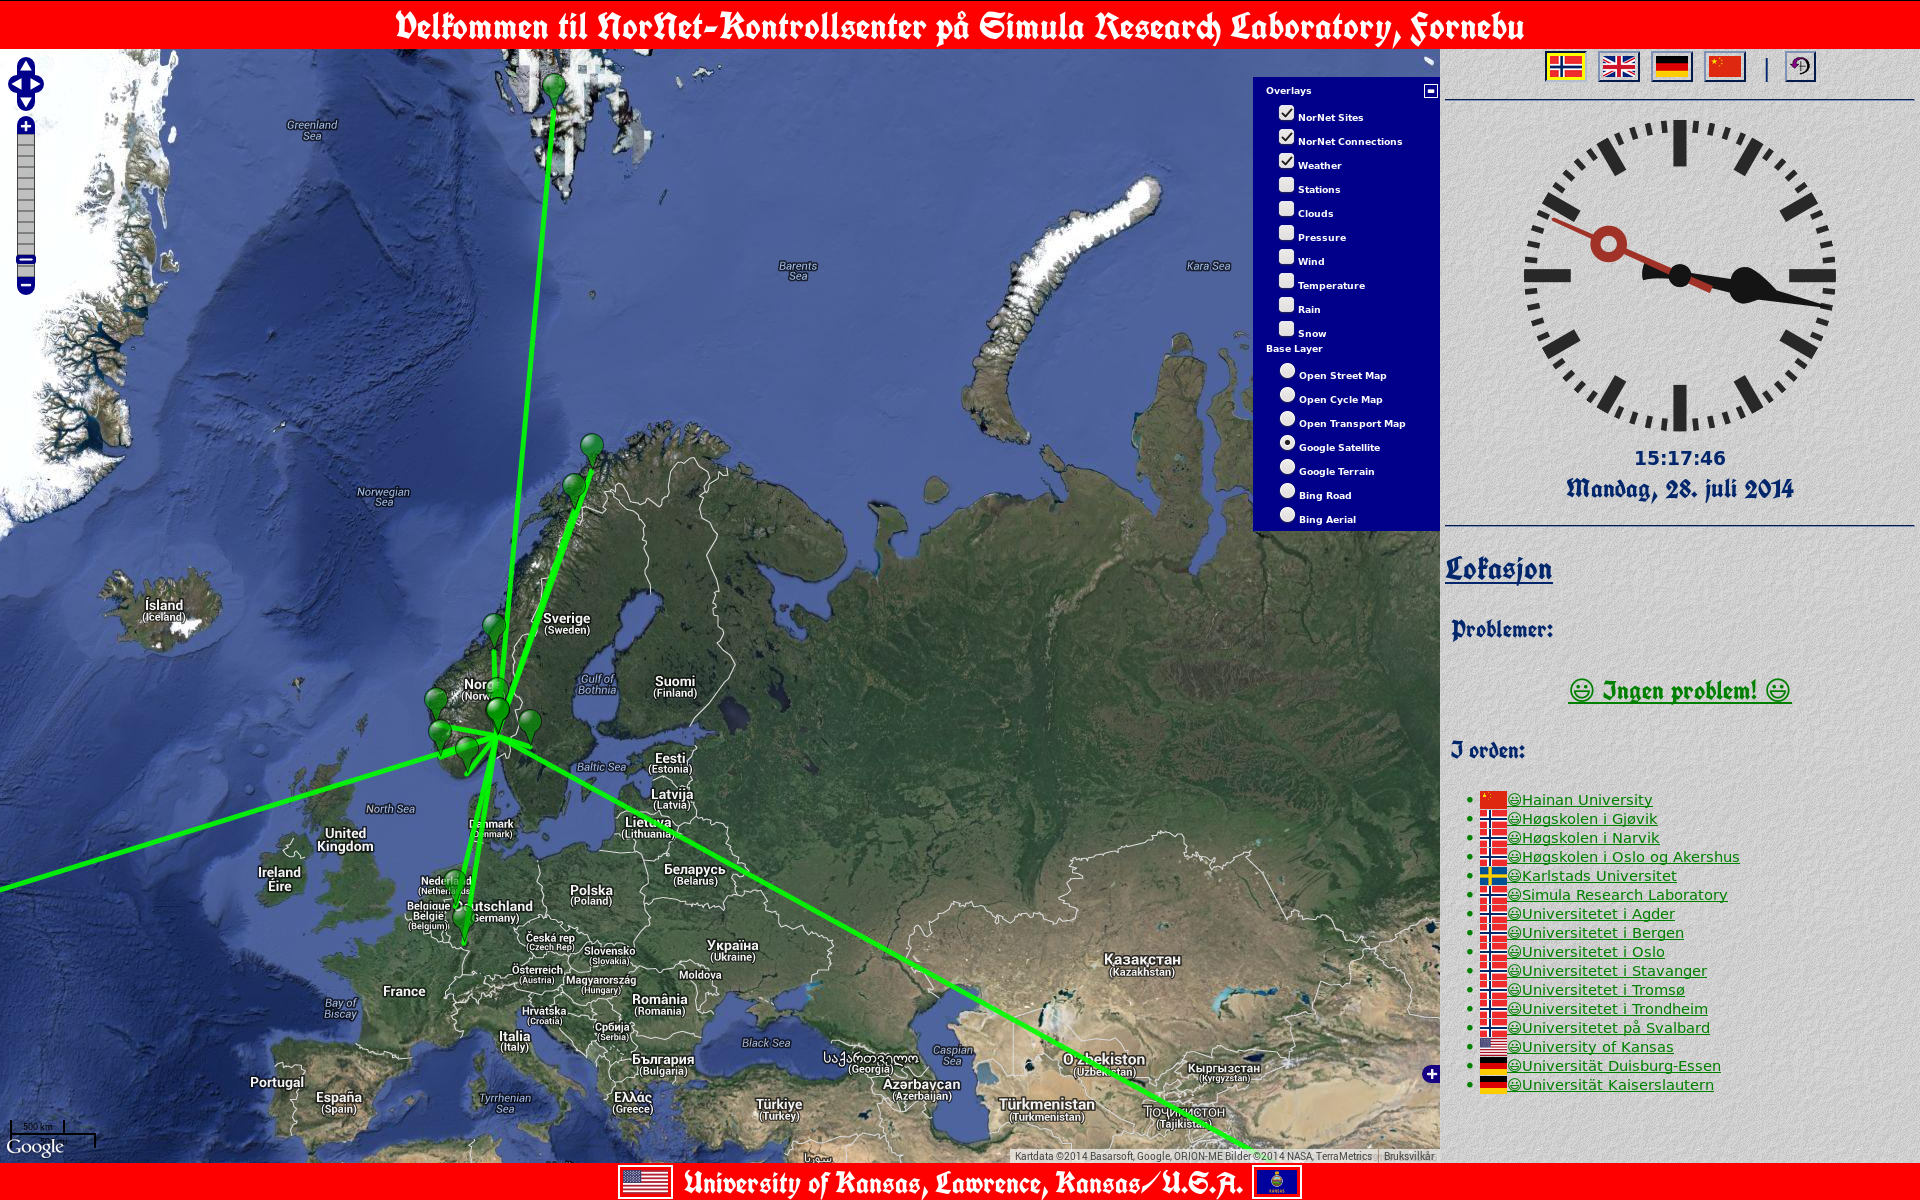
\includegraphics[width=0.98\columnwidth]{%
   Images/PDF/Kontrollsenteret.pdf}
\end{center}
\caption{``NorNet-Kontrollsenter'' -- A Screenshot of the Control Center Display}
\label{cap:Kontrollsenteret}
\end{figure*}
% %%%%%%%%%%%%%%%%%%%%%%%%%%%%%%%%%%%%%%%%%%%%%%%%%%%%%%%%%

In order to achieve the testbed availability described in Section~\ref{sec:Design}, tight monitoring is necessary to detect problems early and to trigger their resolution as soon as possible. The basis of our monitoring infrastructure is a \noun{Nagios}~\cite{NagiosCoreDocumentation} setup, which is deployed in a virtual machine at the Central Site. The ``Monitor'' package provides this functionality, based on the ``Node'' package (see Subsection~\ref{sub:The-Nodes}). \noun{Nagios} actively obtains the status of all components, e.g.\ the systems themselves with \noun{Ping} tests, and services like the PLC's web server by HTTP checks. Particularly, \noun{Nagios} allows a fine-granular configuration of warning and error conditions, as well as the extension to custom services (e.g.\ to check certain system-dependent status values by using SNMP) in form of plug-ins. Such plug-ins have been written to perform checks of sites and tunnels. The monitoring results are recorded by \noun{Nagios}; a web interface provides access for administrators.

While the web interface presents a very detailed and fine-grained view of \noun{NorNet Core}, a more illustrative view was intended to give a quick overview of the site statuses for both administrators and users of the testbed (i.e.\ the researchers). Therefore, we -- as a first step -- applied the \noun{NagMap}\footnote{\noun{NagMap}: \url{https://github.com/hecko/nagmap/}.} plug-in for \noun{Nagios}, which provided a map view of the \noun{NorNet Core} testbed. However, \noun{NagMap} just produced a quite simple projection of the sites and their connections (i.e.\ the tunnels) to a \noun{Google Maps}\footnote{\noun{Google Maps}: \url{https://maps.google.no/}.} satellite map. Particularly due to the fully-connected mesh topology of the tunnels (see Section~\ref{sec:Design}), the link view, however, became relatively confusing. Therefore, we have developed our own plug-in named \noun{NorNet-Kontrollsenter}.

\noun{NorNet-Kontrollsenter} uses \noun{Apache}/PHP~\cite{ApacheDoc} to access the recorded \noun{Nagios} status information. It then provides an HTML page with the results. That is, the plug-in runs on the monitoring system itself. The results can then be accessed from a web server running on the same system, while a web browser on another machine can display the corresponding webpage (as shown in Figure~\ref{cap:Kontrollsenteret}). The returned web page with the results makes use of JavaScript, AJAX (Asynchronous JavaScript and XML) as well as SVG (Scalable Vector Graphics) with JavaScript to provide dynamic updates without having to reload the whole page. Furthermore, instead of tying the map display to a certain map service, we apply \noun{OpenLayers}~\cite{OpenLayersDoc}. It provides a service-independent mapping and layering library in JavaScript; the display can dynamically change between map services (currently, we apply 
\noun{Open Street Map}\footnote{\noun{Open Street Map}: \url{http://www.openstreetmap.org/}.},
\noun{Google Maps} and
\noun{Bing Maps}\footnote{\noun{Bing Maps}: \url{http://www.bing.com/maps/}.}). Furthermore, overlaying functionality is provided. That is, overlays like the \noun{Open Weather Map}\footnote{\noun{Open Weather Map}: \url{http://www.openweathermap.org/}.} overlay can add additional information to the map (in Figure~\ref{cap:Kontrollsenteret}: the current weather as well as clouds and precipitation forecasts). In the future, we plan to use this feature for more detailed network status information. Map services and the visibility of overlays can be changed interactively.

For improved visibility, we only display a connection to the Central Site (in green colour) if all tunnels of a site are working. Only non-working tunnels would result in yellow (warning level) or red (error level) coloured links between sites. Connections to not-yet-deployed sites are represented by grey, dashed lines.

Since the access to the monitoring results is browser-based, it is possible to run multiple browser instances simultaneously. We use this feature e.g.\ to display a map of the Norwegian mainland (see Figure~\ref{cap:Kontrollsenteret}) on a large screen as well as a map of Svalbard (more than 1,000~km north of the mainland) on a separate, small screen. The ``Display'' package extends the ``Node'' setup with configurations for such a display machine, by adding an X~server and the \noun{Firefox} web browser.


% -> mobility support in the future
% -> GUI Localisation



% ###########################################################################
\section{Testbed Deployment and Research Ideas}
% ###########################################################################

Currently, we are in the deployment phase of the sites~\cite{Karlstad2012}. That is, the hardware setup described in Subsection~\ref{sub:The-Sites} has been installed at 7~sites, with 3~further sites in the following weeks.

For the research part of \noun{NorNet Core}, there are obviously use cases for research on resilience (e.g.\ in the context of RSerPool~\cite{IJIIDS2010,Dre2006,rfc-rserpool-overview}, etc.). Furthermore, there is a strong interest in using the testbed in the context of multi-path transport performance with MPTCP~\cite{RBP+11} and CMT-SCTP~\cite{PAMS2012}, as well as for congestion control evaluations~\cite{Globecom2013,ICC2012,YWY08a} in that context. Particularly, there is a growing interest in CMT-SCTP, since \emph{Real-Time Collaboration on the World Wide Web}~(RTCWEB)~\cite{draft-ietf-rtcweb-overview} is based on SCTP. RTCWEB is a framework for browser-to-browser multimedia communications (e.g.\ video conferencing) that is currently under standardisation in the IETF and therefore a very hot research topic. With SCTP being deployed by possibly billions of web browsers on frequently multi-homed endpoints (e.g.\ tablet PCs and smartphones with 3G and WLAN interfaces), the usage of multi-path transport might become very tempting. 



% @@@@@@@@@@@@@@@@@@@@@@@@@@@@@@@@@@@@@@@@@@@@@@@@@@@@@@@@@@@@@@@@@@@@@@@@@@@
\chapter{Getting Access}
\label{cha:Getting-Access}
% @@@@@@@@@@@@@@@@@@@@@@@@@@@@@@@@@@@@@@@@@@@@@@@@@@@@@@@@@@@@@@@@@@@@@@@@@@@

...

% ###########################################################################
\section{User Accounts}
\label{sec:User-Accounts}
% ###########################################################################

PLC

Gatekeeper

Future work



% ###########################################################################
\section{The Gatekeeper}
\label{sec:The-Gatekeeper}
% ###########################################################################

OpenSSH

rsync

tunnel

examples



% ###########################################################################
\section{Kontrollsenteret}
\label{sec:Kontrollsenteret}
% ###########################################################################

...



% ###########################################################################
\section{Further Resources}
% ###########################################################################

% ===========================================================================
\subsection{Mailing Lists}
% ===========================================================================

\url{https://sympa.uio.no/ifi.uio.no/modindex/nornet-announcements}

\url{https://sympa.uio.no/ifi.uio.no/modindex/nornet-users}

...


% ===========================================================================
\subsection{Sites Overview}
% ===========================================================================

\url{https://www.nntb.no/pub/nornet-configuration/NorNetCore-Sites.html}

...



% ###########################################################################
\section{The PLC}
\label{sec:The-PLC}
% ###########################################################################

...

% ===========================================================================
\subsection{Managing the User Account}
\label{sub:Managing-the-Account}
% ===========================================================================

% %%%%%%%%%%%%%%%%%%%%%%%%%%%%%%%%%%%%%%%%%%%%%%%%%%%%%%%%%
\begin{figure*}
\begin{center}
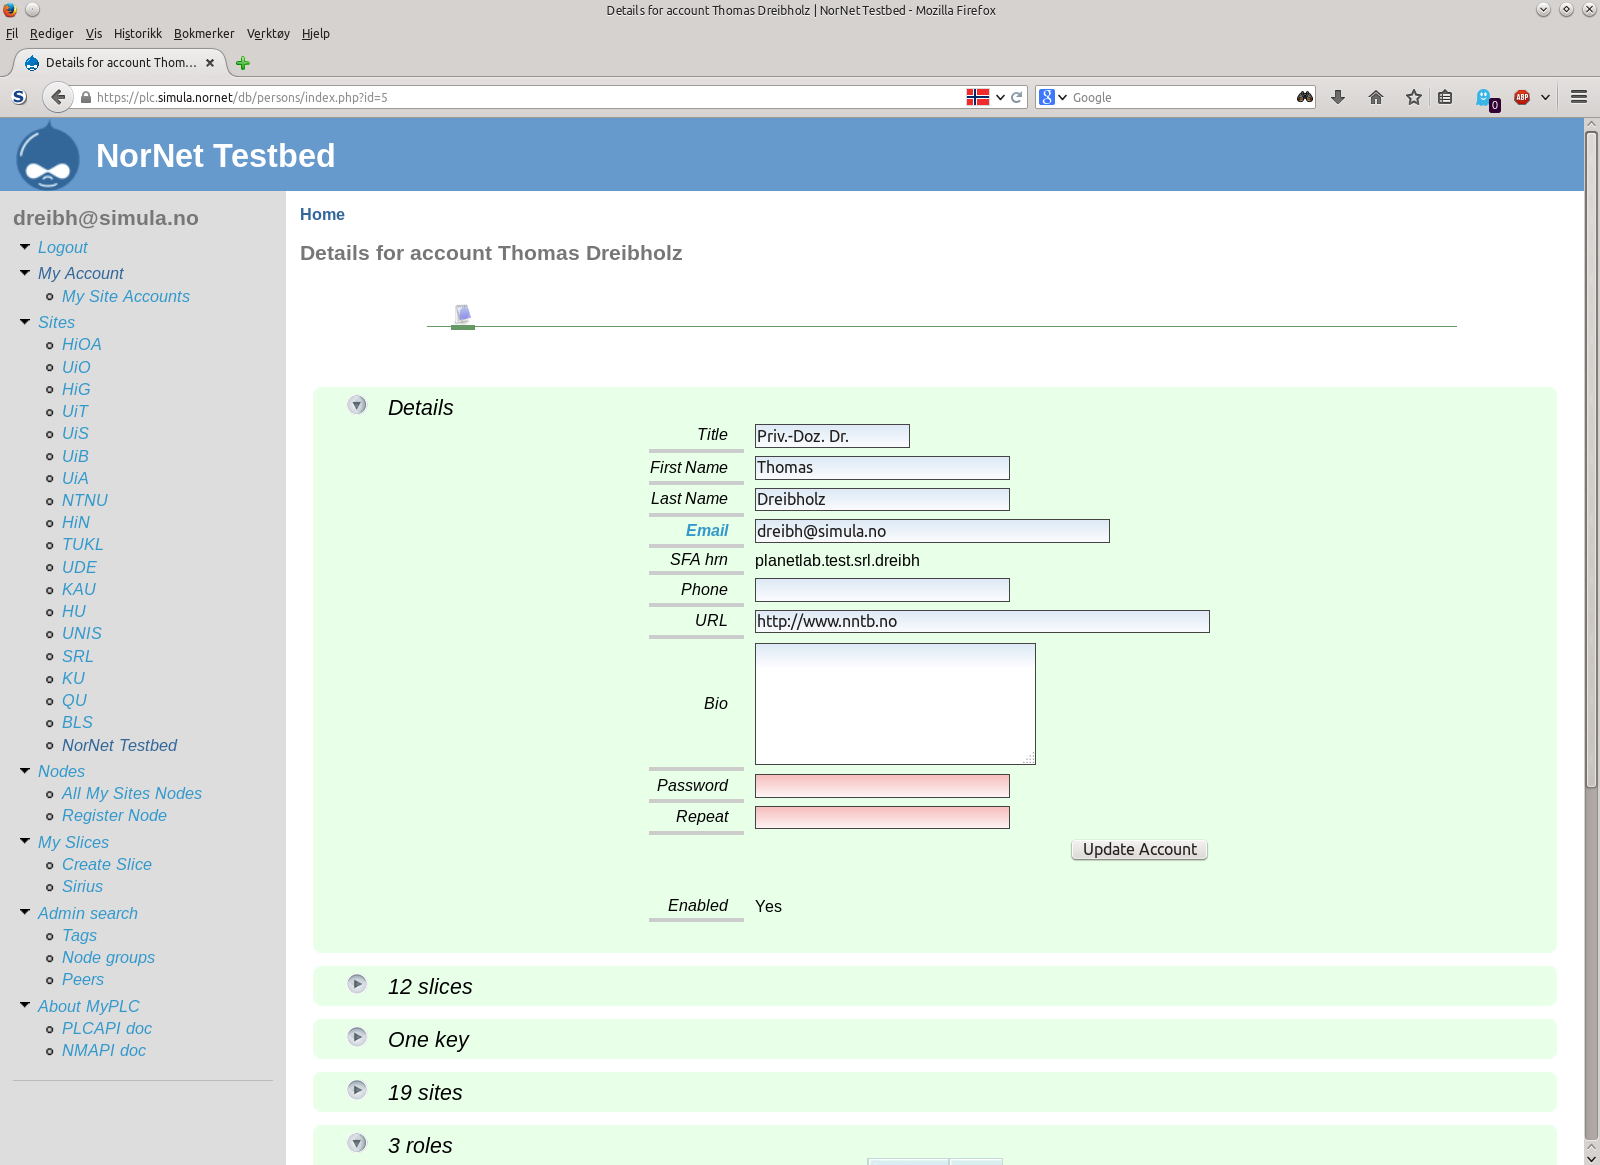
\includegraphics[width=0.90\columnwidth]{Images/PDF/Screenshot-PLC-Account-Details1.pdf}
\end{center}
\caption{The PLC: My Account $\rightarrow$ Details}
\label{cap:PLC-Account-Details-User}
\end{figure*}
% %%%%%%%%%%%%%%%%%%%%%%%%%%%%%%%%%%%%%%%%%%%%%%%%%%%%%%%%%

information

password

key

% %%%%%%%%%%%%%%%%%%%%%%%%%%%%%%%%%%%%%%%%%%%%%%%%%%%%%%%%%
\begin{figure*}
\begin{center}
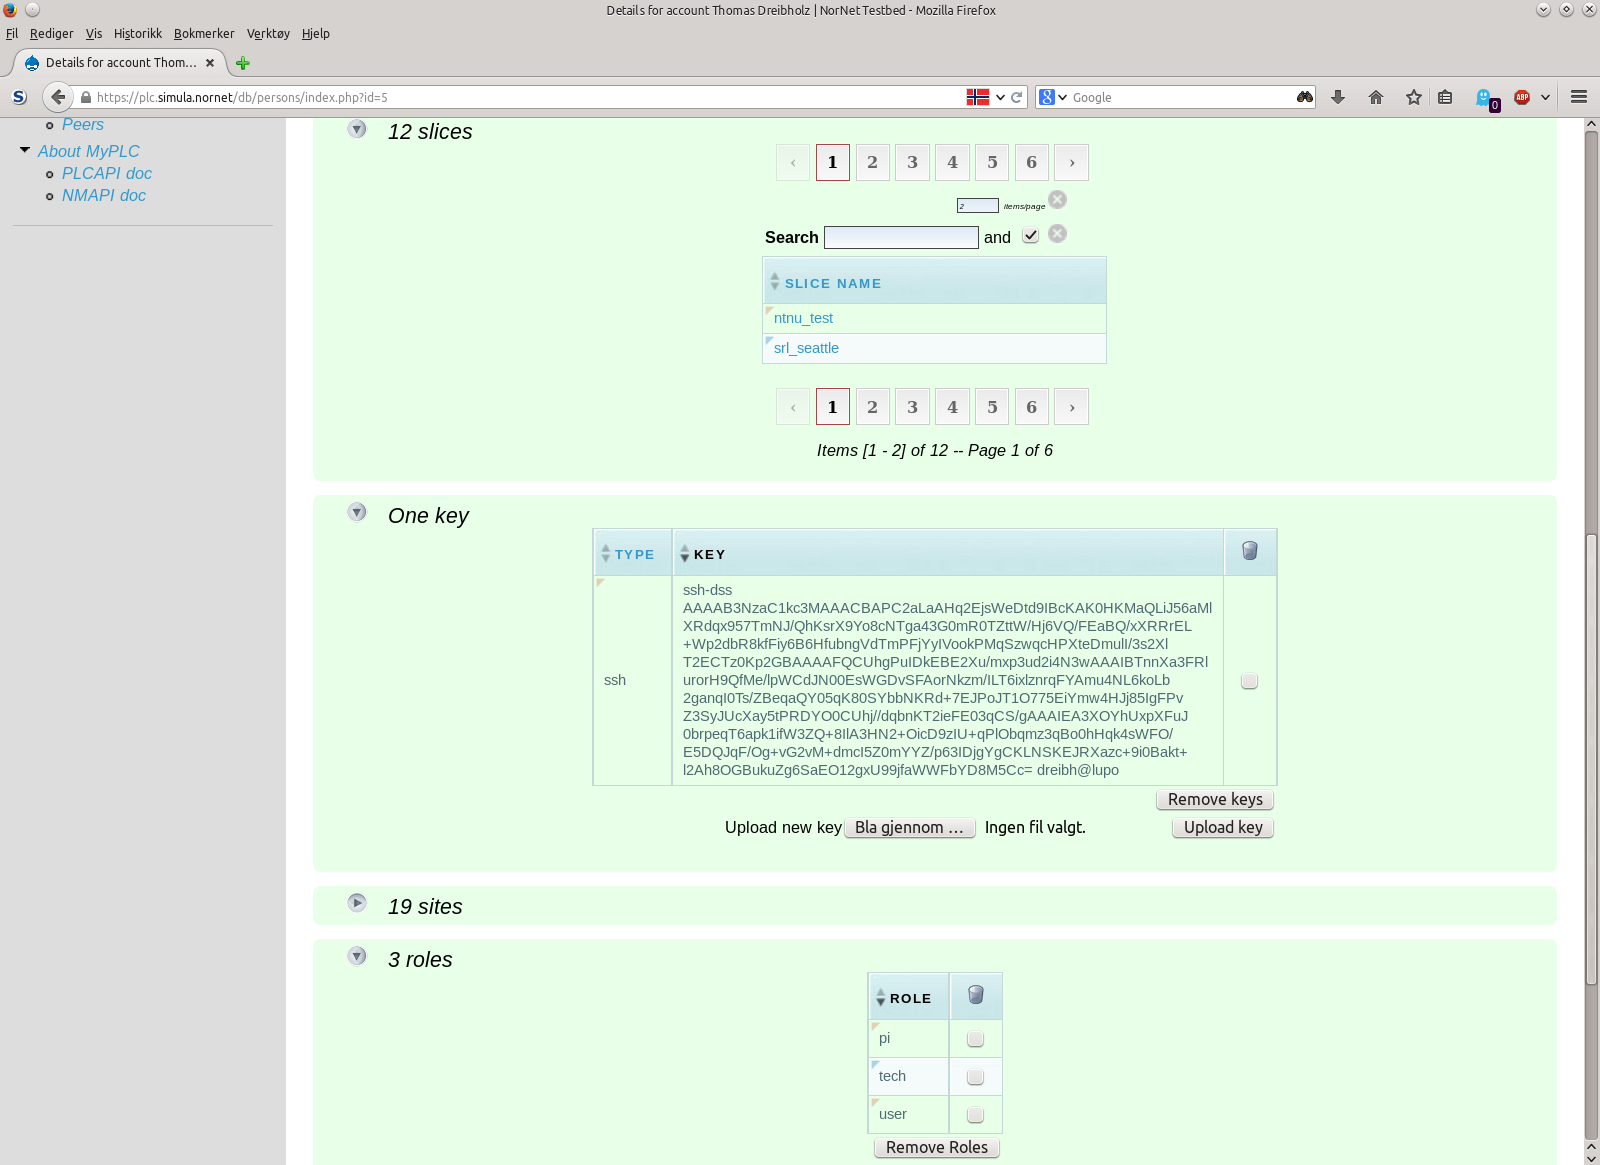
\includegraphics[width=0.90\columnwidth]{Images/PDF/Screenshot-PLC-Account-Details2.pdf}
\end{center}
\caption{My Account $\rightarrow$ Slices, Key and Roles}
\label{cap:PLC-Account-Details-Key-and-Roles}
\end{figure*}
% %%%%%%%%%%%%%%%%%%%%%%%%%%%%%%%%%%%%%%%%%%%%%%%%%%%%%%%%%

...


% ===========================================================================
\subsection{Sites}
\label{sub:Sites}
% ===========================================================================

% %%%%%%%%%%%%%%%%%%%%%%%%%%%%%%%%%%%%%%%%%%%%%%%%%%%%%%%%%
\begin{figure*}
\begin{center}
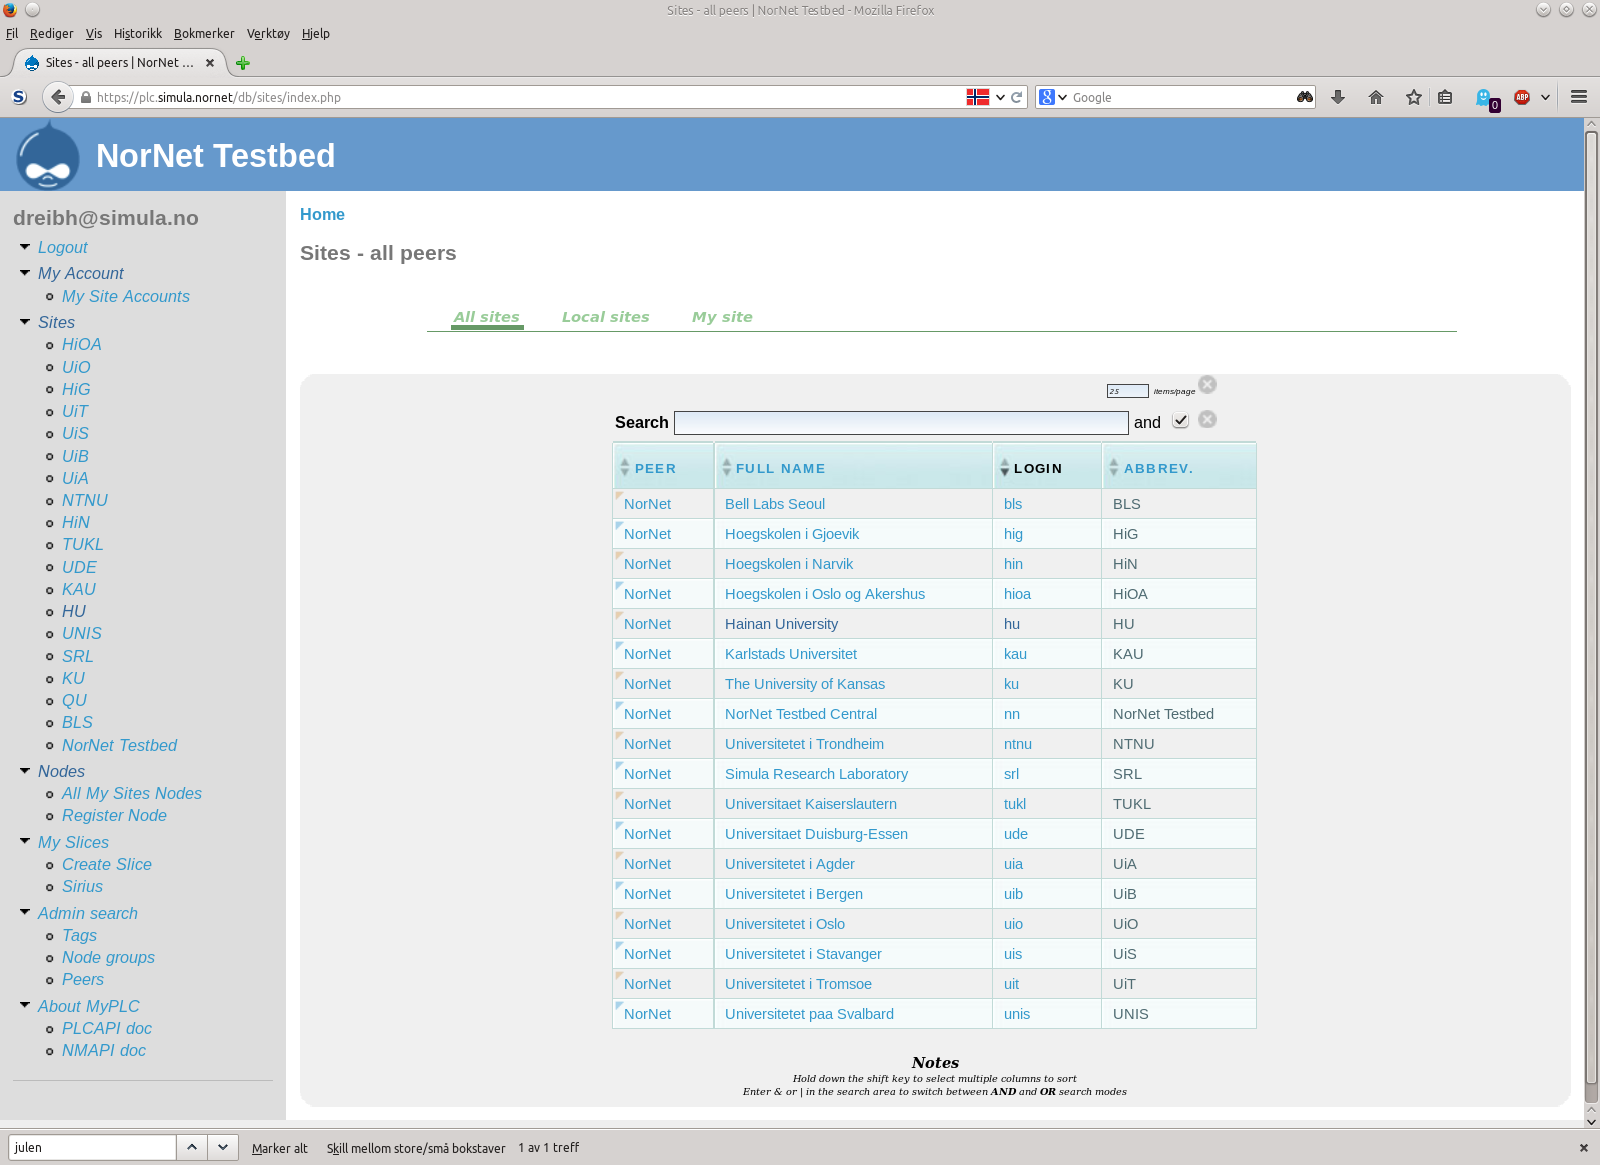
\includegraphics[width=0.90\columnwidth]{%
   Images/PDF/Screenshot-PLC-Sites.pdf}
\end{center}
\caption{Sites}
\label{cap:PLC-Sites}
\end{figure*}
% %%%%%%%%%%%%%%%%%%%%%%%%%%%%%%%%%%%%%%%%%%%%%%%%%%%%%%%%%

% %%%%%%%%%%%%%%%%%%%%%%%%%%%%%%%%%%%%%%%%%%%%%%%%%%%%%%%%%
\begin{figure*}
\begin{center}
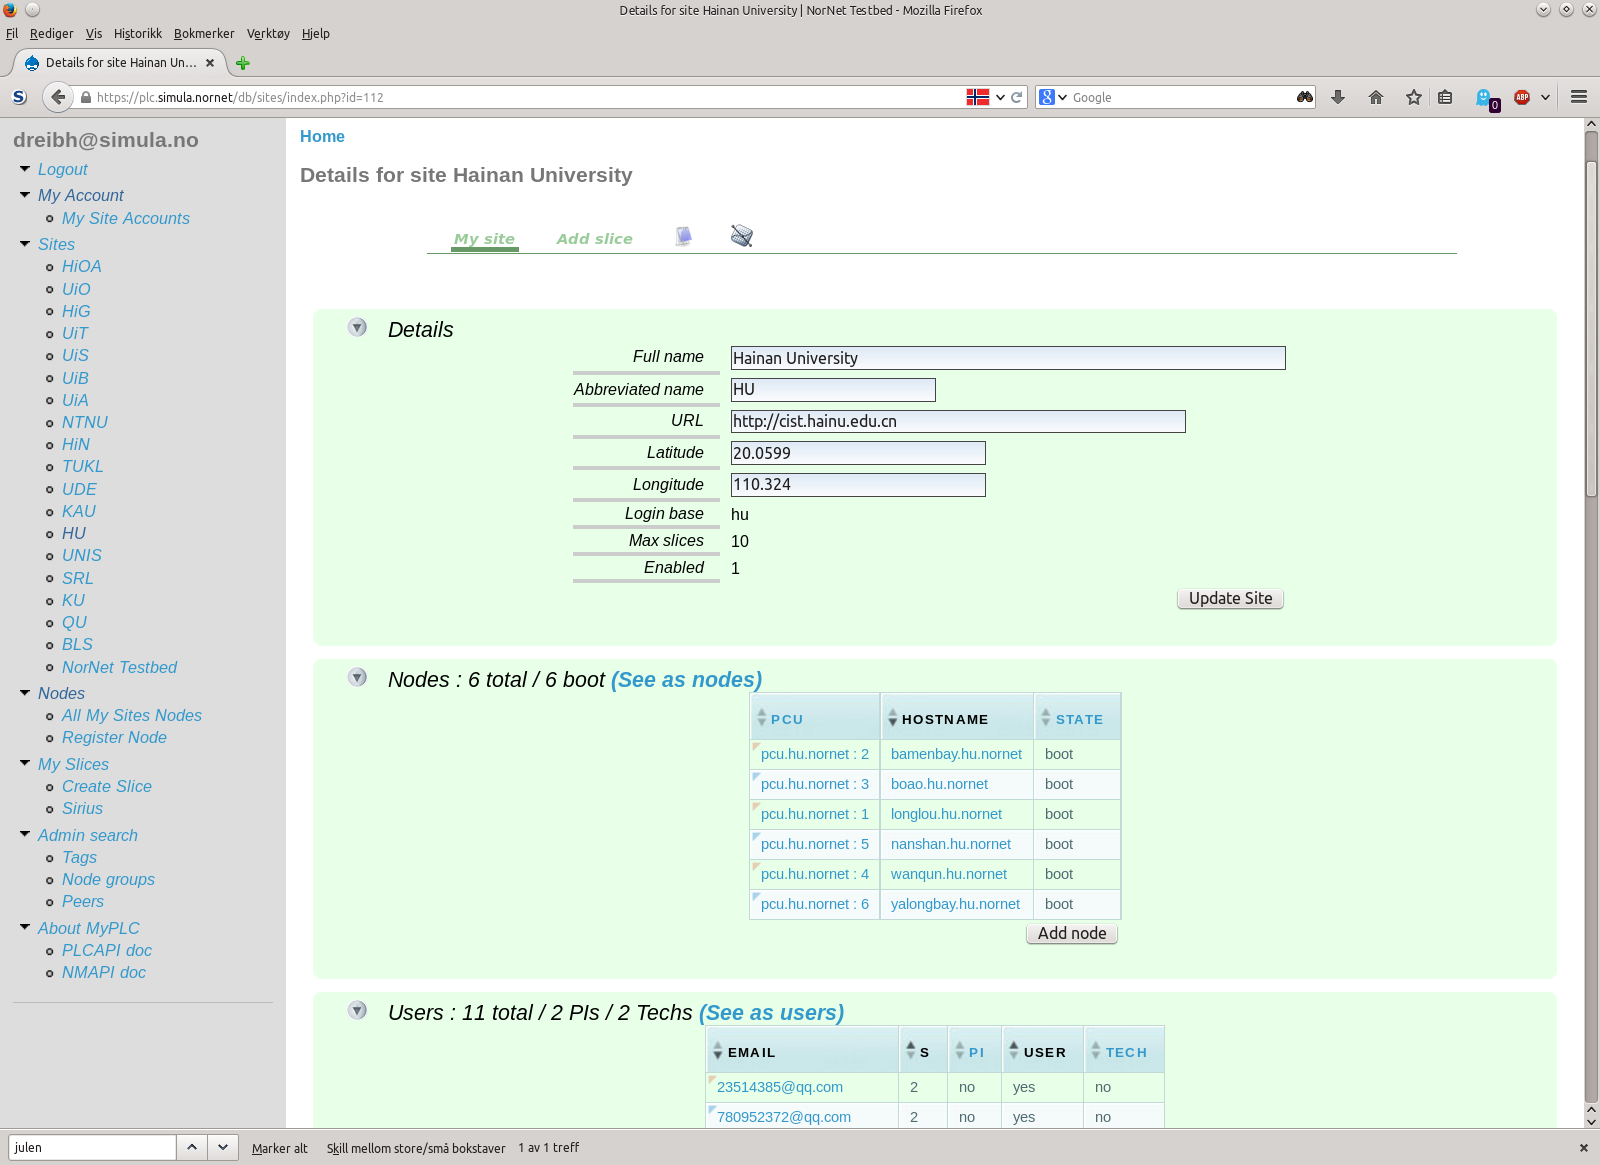
\includegraphics[width=0.90\columnwidth]{%
   Images/PDF/Screenshot-PLC-Sites-HU.pdf}
\end{center}
\caption{Sites $\rightarrow$ Hainan University~(HU)}
\label{cap:PLC-Sites-HU}
\end{figure*}
% %%%%%%%%%%%%%%%%%%%%%%%%%%%%%%%%%%%%%%%%%%%%%%%%%%%%%%%%%

...



% ===========================================================================
\subsection{Nodes}
\label{sub:Nodes}
% ===========================================================================

% %%%%%%%%%%%%%%%%%%%%%%%%%%%%%%%%%%%%%%%%%%%%%%%%%%%%%%%%%
\begin{figure*}
\begin{center}
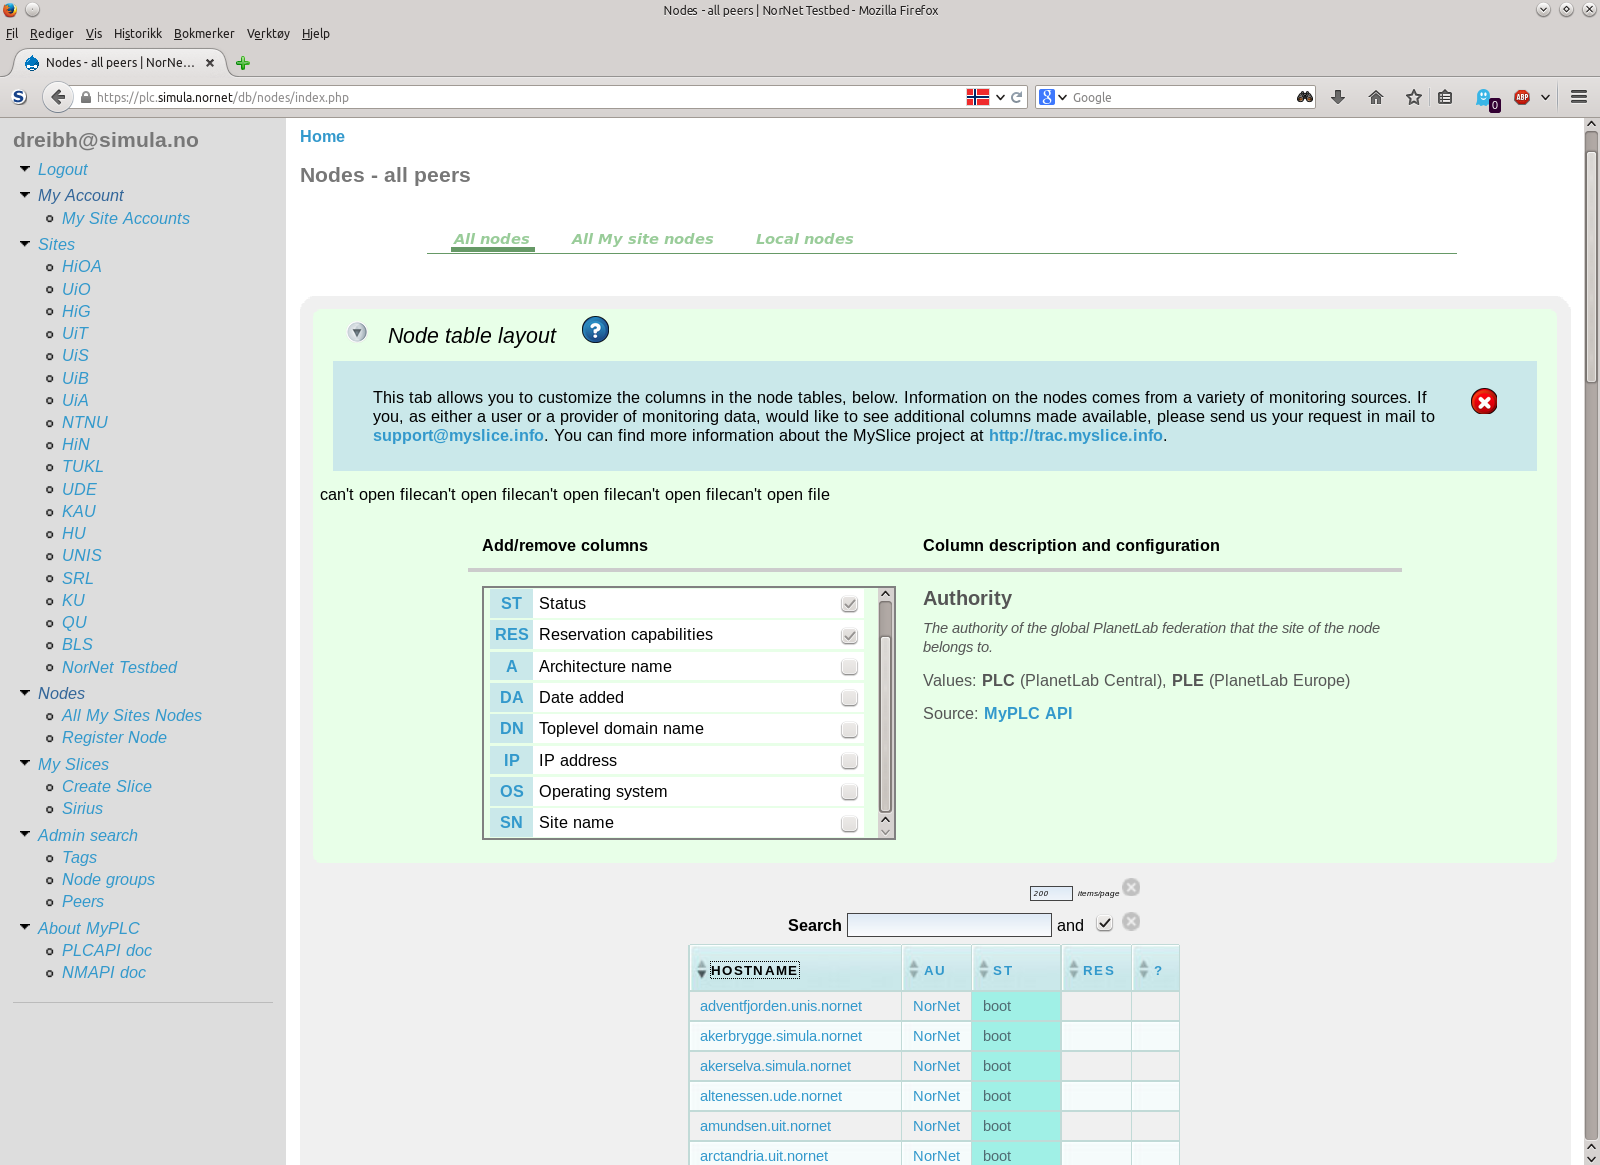
\includegraphics[width=0.90\columnwidth]{%
   Images/PDF/Screenshot-PLC-Nodes.pdf}
\end{center}
\caption{Nodes}
\label{cap:PLC-Nodes}
\end{figure*}
% %%%%%%%%%%%%%%%%%%%%%%%%%%%%%%%%%%%%%%%%%%%%%%%%%%%%%%%%%

% %%%%%%%%%%%%%%%%%%%%%%%%%%%%%%%%%%%%%%%%%%%%%%%%%%%%%%%%%
\begin{figure*}
\begin{center}
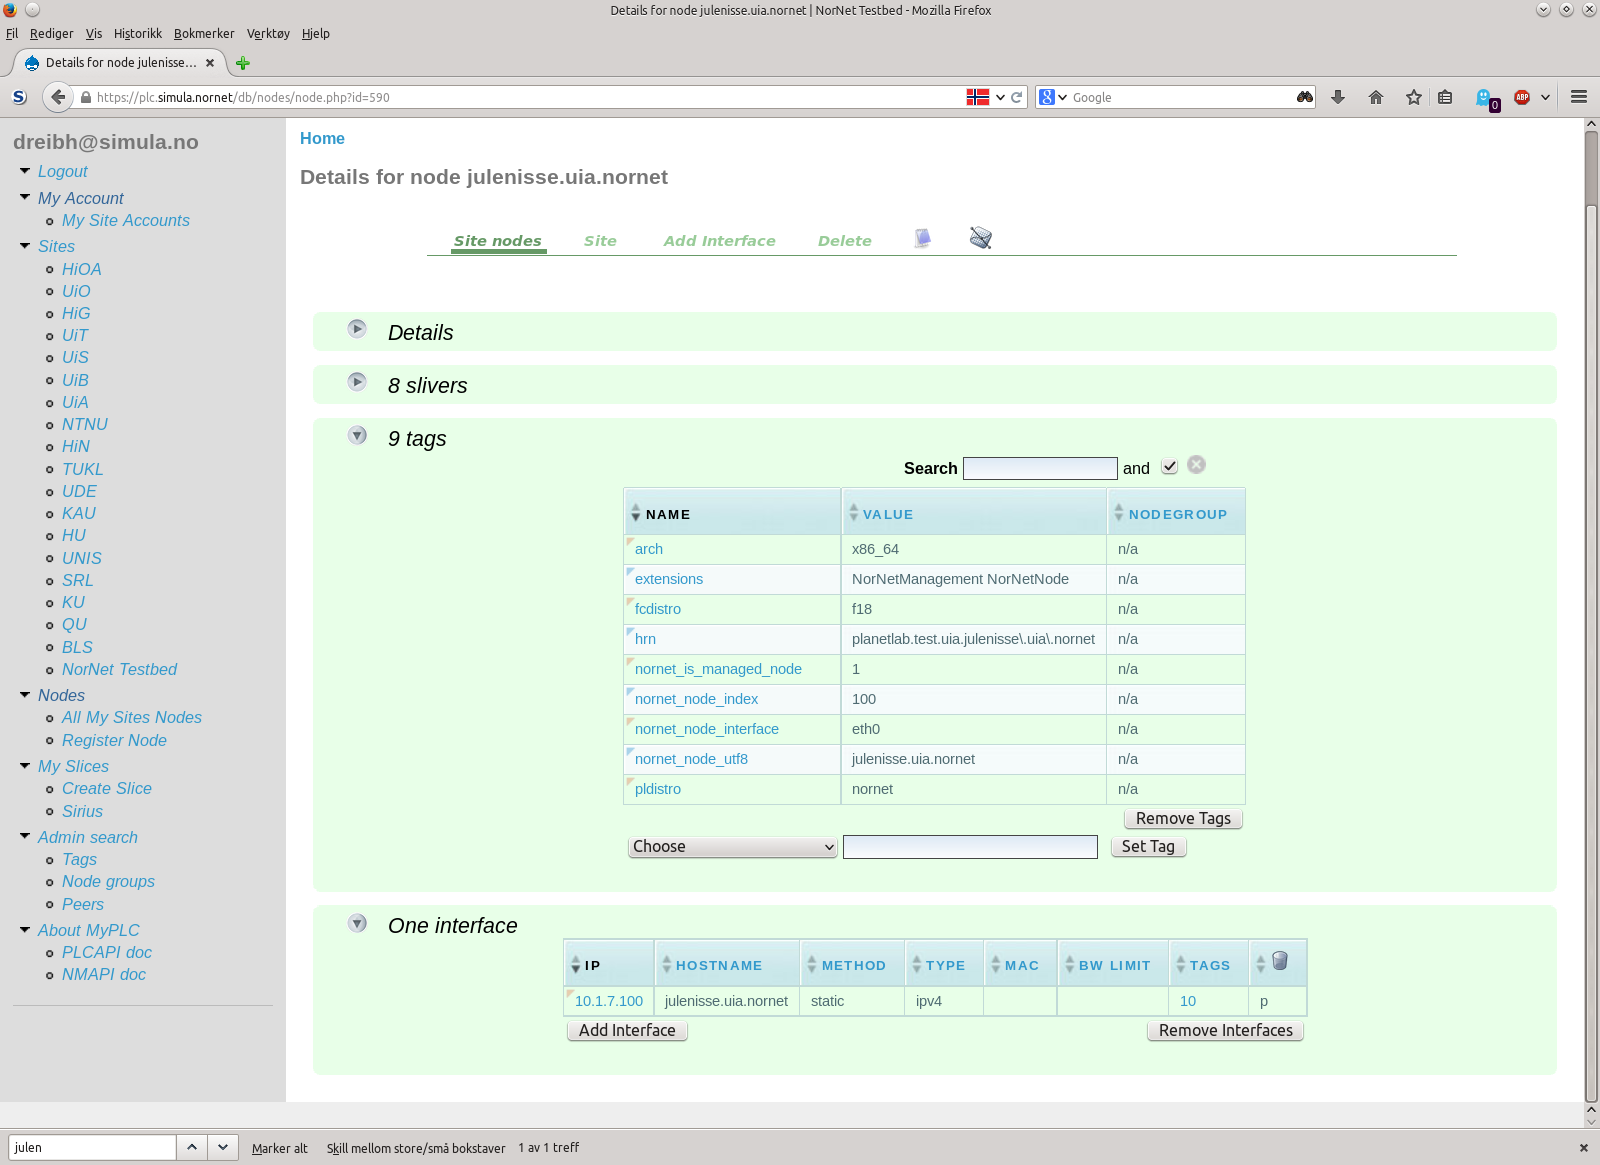
\includegraphics[width=0.90\columnwidth]{%
   Images/PDF/Screenshot-PLC-Node-julenisse.pdf}
\end{center}
\caption{Nodes $\rightarrow$ Node julenisse.uia.nornet}
\label{cap:PLC-Node-Details}
\end{figure*}
% %%%%%%%%%%%%%%%%%%%%%%%%%%%%%%%%%%%%%%%%%%%%%%%%%%%%%%%%%

% %%%%%%%%%%%%%%%%%%%%%%%%%%%%%%%%%%%%%%%%%%%%%%%%%%%%%%%%%
\begin{figure*}
\begin{center}
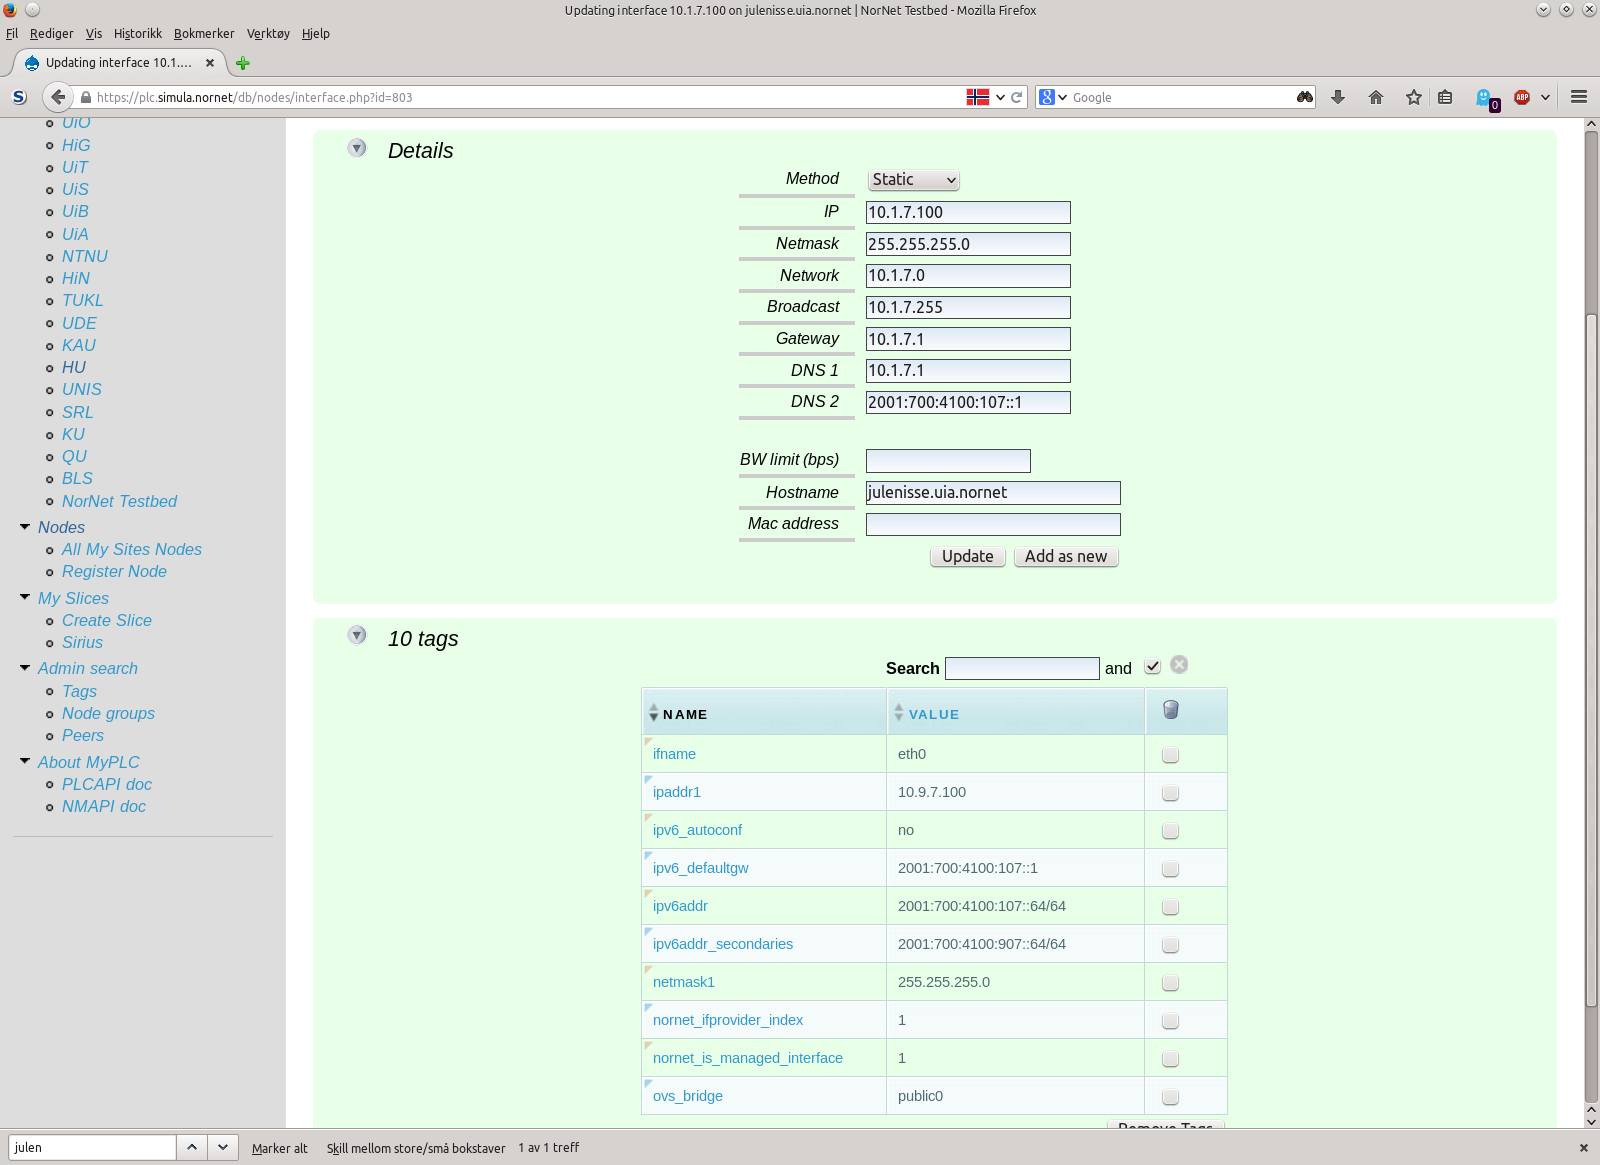
\includegraphics[width=0.90\columnwidth]{%
   Images/PDF/Screenshot-PLC-Node-julenisse-Interface.pdf}
\end{center}
\caption{Nodes $\rightarrow$ Node julenisse.uia.nornet $\rightarrow$ Interface~10.1.7.100}
\label{cap:PLC-Node-Details}
\end{figure*}
% %%%%%%%%%%%%%%%%%%%%%%%%%%%%%%%%%%%%%%%%%%%%%%%%%%%%%%%%%


...


% ===========================================================================
\subsection{Slices and Slivers}
\label{sub:Slices-and-Slivers}
% ===========================================================================

...



% ###########################################################################
\section{Graphite, etc.}
\label{sec:...}
% ###########################################################################

...



% @@@@@@@@@@@@@@@@@@@@@@@@@@@@@@@@@@@@@@@@@@@@@@@@@@@@@@@@@@@@@@@@@@@@@@@@@@@
\chapter{The Research Nodes}
\label{cha:Research-Nodes}
% @@@@@@@@@@@@@@@@@@@@@@@@@@@@@@@@@@@@@@@@@@@@@@@@@@@@@@@@@@@@@@@@@@@@@@@@@@@

...

% ###########################################################################
\section{Logging In}
\label{sec:Logging-In}
% ###########################################################################

...

ssh and keys



% ###########################################################################
\section{Installing Software}
\label{sec:Installing-Software}
% ###########################################################################

yum ...

gcc, etc.

...


% ###########################################################################
\section{Using Multi-Homing}
\label{sec:Using-Multi-Homing}
% ###########################################################################

ping and traceroute examples

NetPerfMeter!

...


% ###########################################################################
\section{Using Multi-Path TCP}
\label{sec:Using-Multi-Path-TCP}
% ###########################################################################

the patch

options

...



% @@@@@@@@@@@@@@@@@@@@@@@@@@@@@@@@@@@@@@@@@@@@@@@@@@@@@@@@@@@@@@@@@@@@@@@@@@@
\chapter{Custom Configuration Possibilities}
\label{cha:Custom-Configuration-Possibilities}
% @@@@@@@@@@@@@@@@@@@@@@@@@@@@@@@@@@@@@@@@@@@@@@@@@@@@@@@@@@@@@@@@@@@@@@@@@@@

...


% ###########################################################################
\section{Custom Virtual Machines}
\label{sec:Custom-Virtual-Machines}
% ###########################################################################

...


% ###########################################################################
\section{Custom Routing Rules}
\label{sec:Custom-Routing-Rules}
% ###########################################################################

SIP Honeypot project~\cite{IFIPNetworking2014}

...



% ###########################################################################
\section{Summary}
% ###########################################################################

...
